\graphicspath{{./figures/arquitectura/}}

\section{Arquitectura del Sistema}

Esta sección describe los componentes principales del sistema, sus responsabilidades e interacciones, así como las tecnologías propuestas para su implementación.

\vspace{1cm}

\begin{figure}[H]
    \centering
    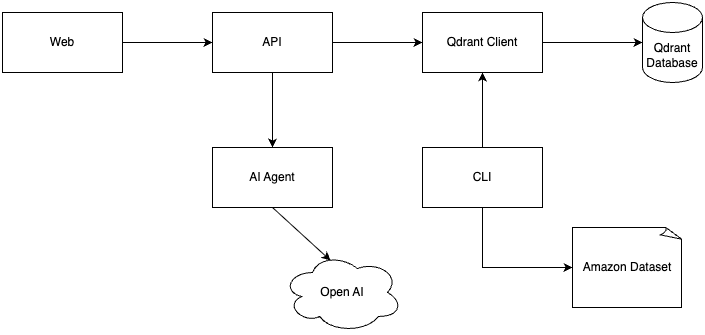
\includegraphics[width=0.8\textwidth]{architecture.png}
    \caption{Diagrama de alto nivel de la arquitectura del sistema.}
    \label{fig:system_architecture}
\end{figure}

\subsection{Web}

El componente Web constituye la interfaz de usuario principal del sistema, proporcionando una experiencia de usuario moderna e interactiva para la búsqueda y exploración de productos. La aplicación implementa URLs compartibles donde todos los parámetros de búsqueda y filtrado están codificados en la URL, permitiendo a los usuarios compartir resultados específicos y reproducir exactamente los mismos resultados.

Se eligió \href{https://nextjs.org/}{Next.js 15}~\cite{NextJS} con React por la experiencia previa del equipo y las ventajas que ofrece para optimizar el tiempo de las consultas. Next.js 15 ofrece funcionalidades avanzadas en el App Router, como Server Components y Server Actions que fueron aprovechadas para mejorar el rendimiento y la experiencia de usuario.

\subsection{API}

Este componente constituye la capa de servicios que comunica el frontend con los distintos motores de búsqueda y recomendación. Incluye endpoints para listar productos (recibiendo parámetros de filtros y búsqueda), obtener información detallada de productos específicos, gestionar conversaciones con el agente AI, y generar recomendaciones de productos.

Se implementó utilizando \href{https://fastapi.tiangolo.com/}{FastAPI}~\cite{FastAPI}, un framework moderno de Python que permite un desarrollo eficiente y robusto. La decisión se basó en su sencillez y la simple integración con LangGraph para la implementación del módulo Agent. FastAPI ofrece validación automática de datos mediante \href{https://docs.pydantic.dev/latest/}{Pydantic}~\cite{Pydantic}, tipado estático que reduce errores en tiempo de desarrollo, y documentación automática con OpenAPI que sirvió como recurso valioso para la paralelización del desarrollo API-Frontend.

\subsection{Agent}

El módulo Agent implementa un asistente AI conversacional que interactúa con los usuarios para entender sus preferencias y necesidades, realizar búsquedas de productos, y presentar resultados de manera contextual y útil.

Se implementó utilizando \href{https://langchain-ai.github.io/langgraph/}{LangGraph}~\cite{LangGraph}, un framework para construir aplicaciones de AI con flujos de trabajo complejos y estados persistentes. La elección se basó en su capacidad para manejar conversaciones multi-turno y mantener el contexto del usuario a lo largo de la interacción. El agente implementa un grafo de estados que incluye nodos para la recolección de preferencias, búsqueda de productos y presentación de resultados, utilizando \href{https://openai.com/}{OpenAI GPT-4}~\cite{OpenAI} para el procesamiento del lenguaje natural y la generación de respuestas contextuales.

\subsection{Qdrant Client}

El Qdrant Client es el componente responsable de la gestión de la base de datos vectorial y la implementación de búsquedas híbridas que combinan múltiples estrategias para maximizar la relevancia de los resultados.

Se decidió utilizar \href{https://qdrant.tech/}{Qdrant}~\cite{Qdrant} como base de datos vectorial por su funcionalidad avanzada para la búsqueda híbrida de productos. Qdrant ofrece capacidades únicas que fueron aprovechadas en el sistema: búsqueda híbrida que combina embeddings densos (para capturar significado semántico) y esparsos (para coincidencias textuales precisas), modelos de embeddings integrados utilizando \href{https://github.com/qdrant/fastembed}{fastembed}~\cite{FastEmbed} con modelos optimizados, filtrado avanzado que permite filtrar resultados por categorías, precios y otros atributos, y reranking para mejorar la calidad de los resultados.

\subsection{CLI}

La interfaz de línea de comandos (CLI) proporciona una herramienta de administración y desarrollo que facilita la carga de datos, el testeo de funcionalidades, y la gestión del sistema.

Se implementó utilizando \href{https://typer.tiangolo.com/}{Typer}~\cite{Typer}, una biblioteca moderna de Python para crear aplicaciones de línea de comandos. La elección se basó en su simplicidad, integración con FastAPI (ambos creados por el mismo autor), y su capacidad para generar documentación automática de comandos. La CLI resultó muy útil tanto para la carga de datos como para el testeo previo al desarrollo de los endpoints API, proporcionando funcionalidades como gestión de colecciones, carga de datos, búsqueda de productos, administración de productos y testeo de conexión. Utiliza \href{https://rich.readthedocs.io/}{Rich}~\cite{Rich} para proporcionar una interfaz visual atractiva con tablas formateadas, barras de progreso, y mensajes de estado coloridos.

\subsection{Dataset}

Para la información de productos, se utilizó el conjunto de datos de Amazon disponible en \href{https://www.kaggle.com/datasets/lokeshparab/amazon-products-dataset/data?select=Amazon-Products.csv}{Kaggle}~\cite{Amazon}. Este conjunto de datos ofrece una amplia variedad de atributos por producto, incluyendo:

\begin{itemize}
    \item Título y descripción detallada
    \item Categorías y subcategorías
    \item Precio y disponibilidad
    \item Valoraciones y número de reseñas
    \item Imágenes de productos
    \item Especificaciones técnicas
\end{itemize}

La riqueza de estos atributos permitió implementar las modalidades de búsqueda previamente mencionadas, así como proporcionar información detallada para el agente AI y el sistema de recomendaciones.
